\subsection{Average Treatment Effect}
\begin{table}[htbp]
\centering

\begin{minipage}[t]{0.48\textwidth}
\centering
\caption{Main estimation results}
\label{tab:main_results}
\footnotesize
\begin{tabular}{@{}lcc@{}}
\toprule
Model & ATE & 95\% CI \\
\midrule
GWL baseline (HC3) & -0.0263 & [-0.0304, -0.0222] \\
GWL extended (HC3) & -0.0260 & [-0.0302, -0.0218] \\
LinearDML & -0.0241 & [-0.0282, -0.0200] \\
CausalForestDML & -0.0244 & [-0.0454, -0.0034] \\
\bottomrule
\end{tabular}
\end{minipage}
\hfill
\begin{minipage}[t]{0.48\textwidth}
\centering
\begin{threeparttable}
\caption{Repeated-split BLP heterogeneity test}
\label{tab:blp_results}
\footnotesize
\begin{tabular}{@{}lcc@{}}
\toprule
Term & Estimate & 95\% CI \\
\midrule
ATE ($\beta_1$) & -0.0236 & [-0.0288, -0.0185] \\
Heterogeneity loading ($\beta_2$) & 0.6703 & [0.3326, 1.0012] \\
\bottomrule
\end{tabular}
\begin{tablenotes}[flushleft]
\footnotesize
\item Estimates are medians across 100 repeated sample splits.
\end{tablenotes}
\end{threeparttable}
\end{minipage}

\end{table}


\subsection{Heterogeneous Treatment Effects}

\begin{figure}[htbp]
\centering
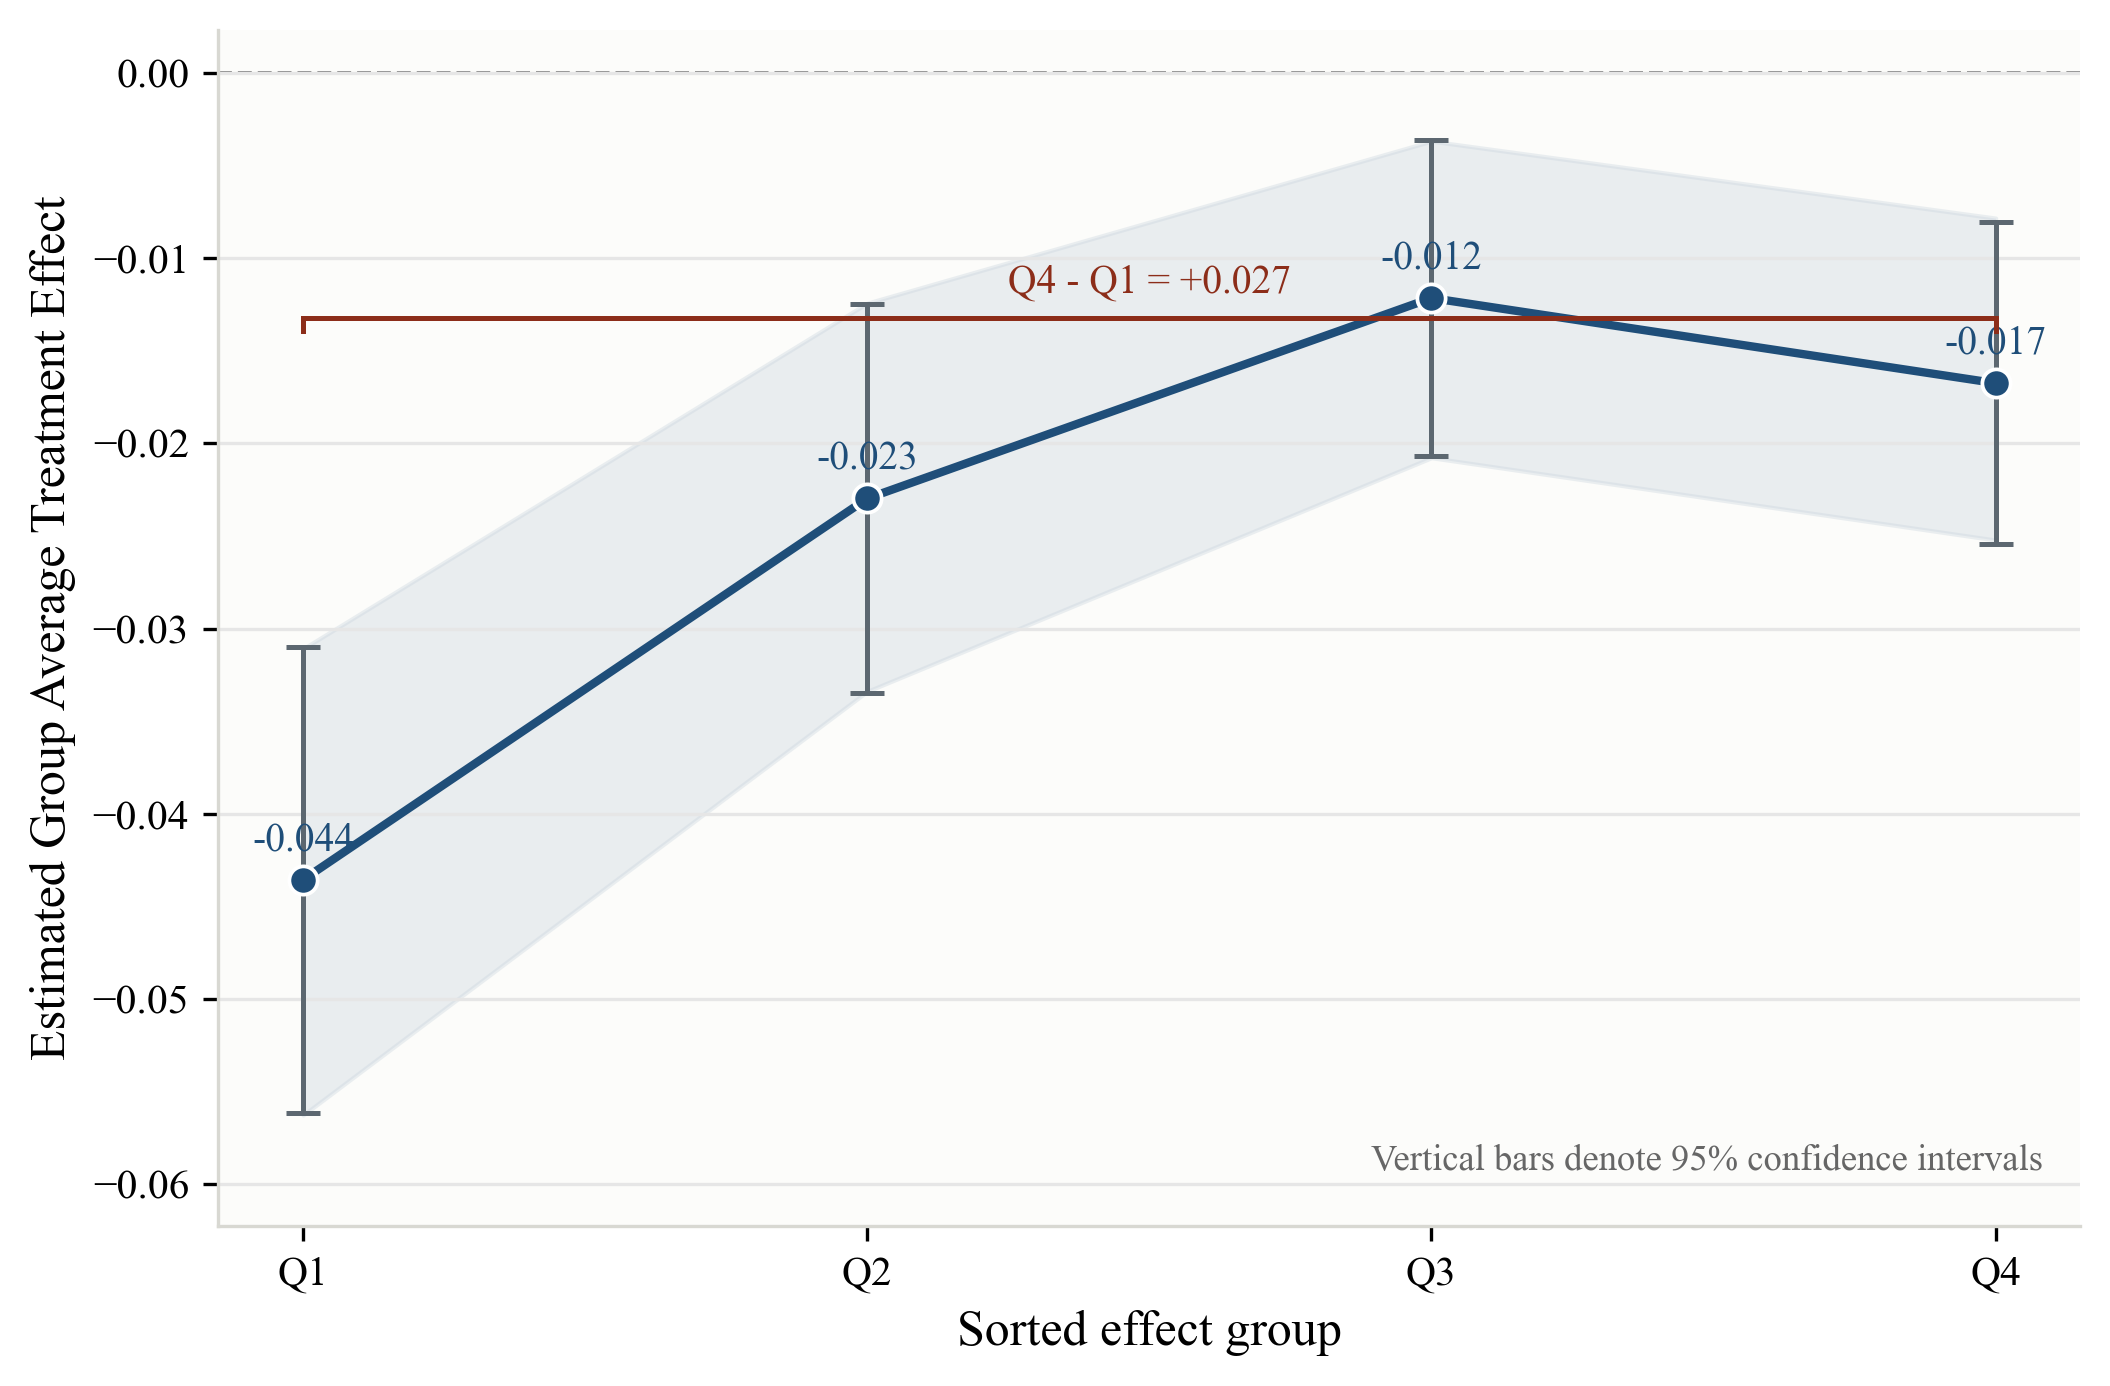
\includegraphics[width=0.72\textwidth]{latex/repeated_split_sorted_gate_plot.png}
\caption{Repeated-split sorted group average treatment effects. The most affected group (Q1) exhibits a substantially more negative treatment effect than the least affected group (Q4), indicating economically meaningful heterogeneity. Vertical bars denote 95\% confidence intervals.}
\label{fig:repeated_gate}
\end{figure}

\subsubsection*{CLAN and Covariate Profiles}
\begin{table}[htbp]
\centering
\begin{threeparttable}
\caption{Repeated-split CLAN comparison between the most affected group (Q1) and the least affected group (Q4)}
\label{tab:clan_results}
\footnotesize
\begin{tabular*}{\textwidth}{@{\extracolsep{\fill}}lcccc@{}}
\toprule
Characteristic & Q1 & Q4 & Diff.\ (Q4$-$Q1) & 95\% CI \\
\midrule
Food share & 0.441 & 0.320 & -0.119 & [-0.127, -0.111] \\
Log total expenditure & 12.864 & 13.930 & 1.067 & [1.037, 1.096] \\
Age & 63.233 & 45.440 & -17.493 & [-18.117, -16.889] \\
Household size & 2.276 & 4.677 & 2.405 & [2.336, 2.474] \\
Male share & 0.710 & 0.954 & 0.242 & [0.225, 0.260] \\
Propensity score & 0.453 & 0.597 & 0.144 & [0.138, 0.150] \\
\bottomrule
\end{tabular*}
\begin{tablenotes}[flushleft]
\footnotesize
\item Notes: Q1 denotes the most affected group and Q4 the least affected group. Entries report median group means across repeated sample splits. The final column reports the 95\% confidence interval for the difference between Q4 and Q1.
\end{tablenotes}
\end{threeparttable}
\end{table}


\subsubsection*{Permutation Importance}
\begin{figure}[htbp]
\centering
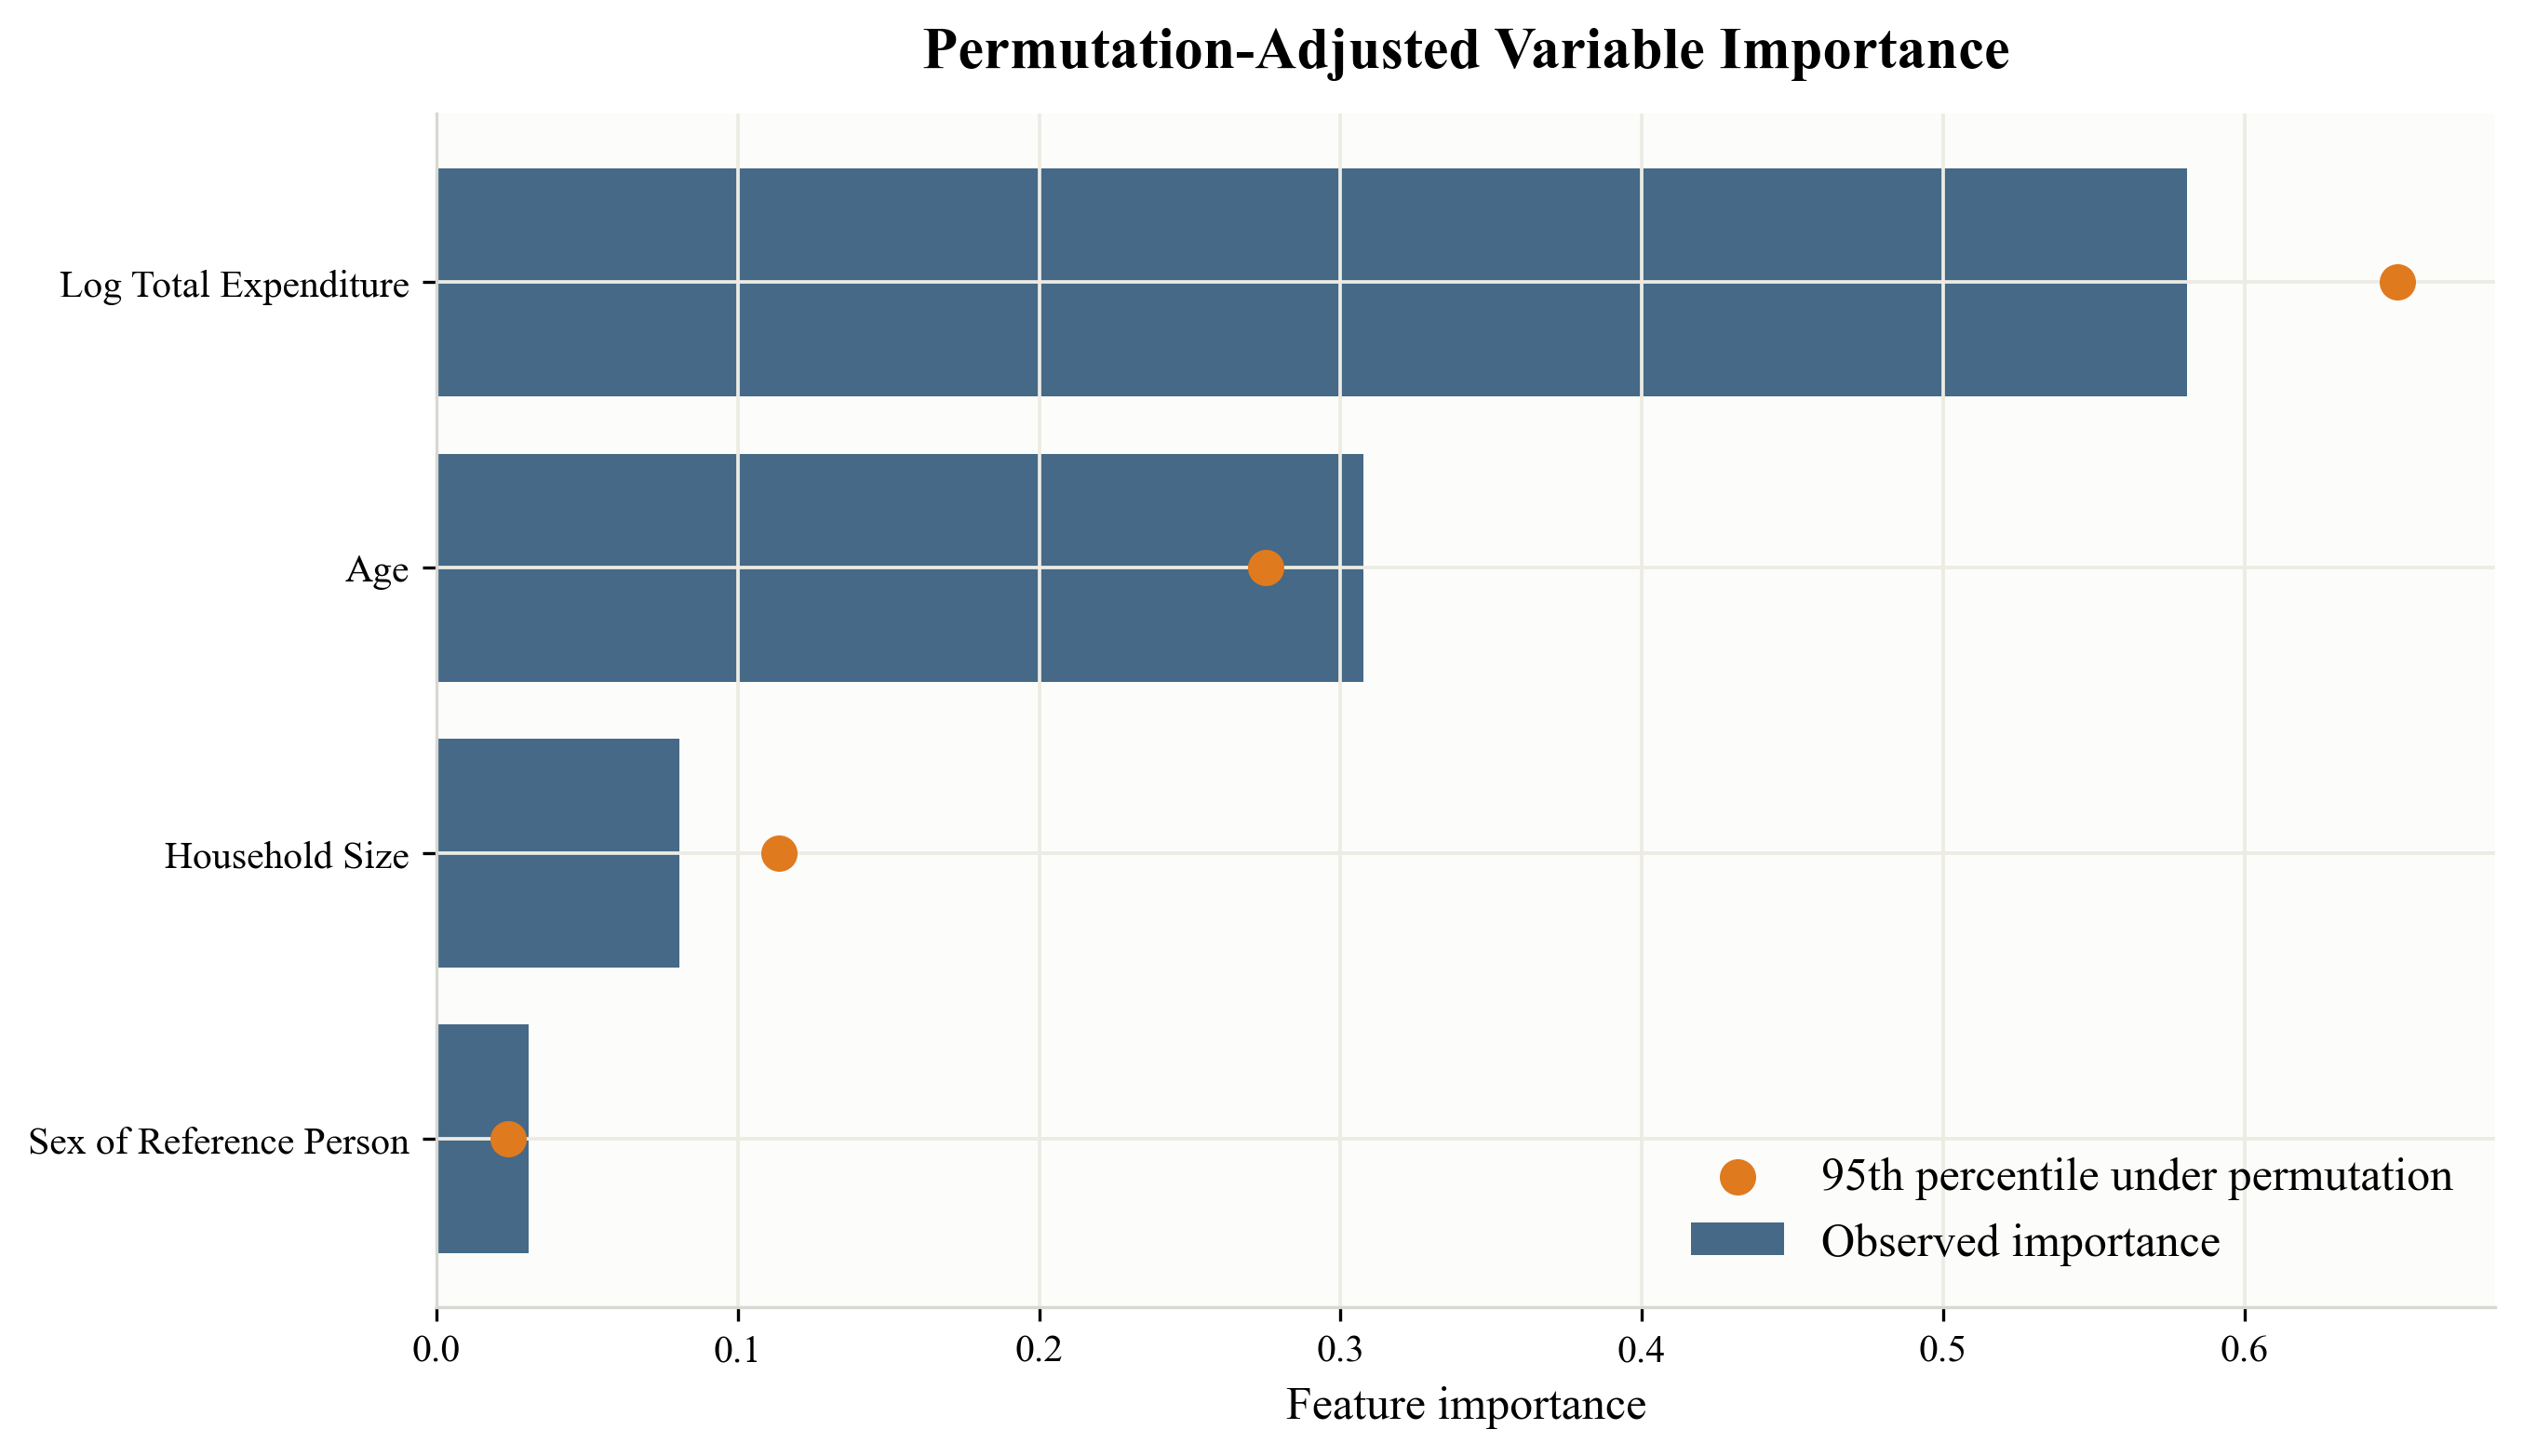
\includegraphics[width=0.72\textwidth]{latex/permutation_importance_plot.png}
\caption{Permutation-adjusted variable importance from the repeated-split heterogeneity analysis. Higher observed importance relative to the permutation benchmark indicates more robust evidence that a covariate contributes to treatment-effect heterogeneity.}
\label{fig:perm_importance}
\end{figure}

\begin{table}[htbp]
\centering
\begin{threeparttable}
\caption{Permutation-adjusted variable importance}
\label{tab:perm_results}
\footnotesize
\begin{tabular*}{\textwidth}{@{\extracolsep{\fill}}lccccc@{}}
\toprule
Variable & Observed & Perm.\ median & Perm.\ 95th pct. & $p$-value & $-\log(p)$ \\
\midrule
Log total expenditure & 0.581 & 0.631 & 0.655 & 1.000 & 0.000 \\
Age & 0.308 & 0.257 & 0.274 & 0.020 & 3.932 \\
Household size & 0.081 & 0.092 & 0.120 & 0.980 & 0.020 \\
Male share & 0.031 & 0.019 & 0.026 & 0.020 & 3.932 \\
\bottomrule
\end{tabular*}
\begin{tablenotes}[flushleft]
\footnotesize
\item Notes: The table compares observed score-based forest importance with the permutation benchmark. Smaller $p$-values indicate stronger evidence that observed importance exceeds what could arise under random permutation of the heterogeneity score.
\end{tablenotes}
\end{threeparttable}
\end{table}

